\section{Introduction}

\subsection{Radio interferometry system}\label{intro:sys}
This project is focused on distributing image Reconstruction for radio interferometers, which is only one of three steps in the pipeline from measurements to the final image. We give a quick overview over the whole pipeline in figure \ref{intro:system} and how Radio Interferometers work in principle: The antennas observe the arriving electromagnetic wave, gets processed in three steps, correlation, calibration and image reconstruction. 

\begin{figure}[h]
	\centering
	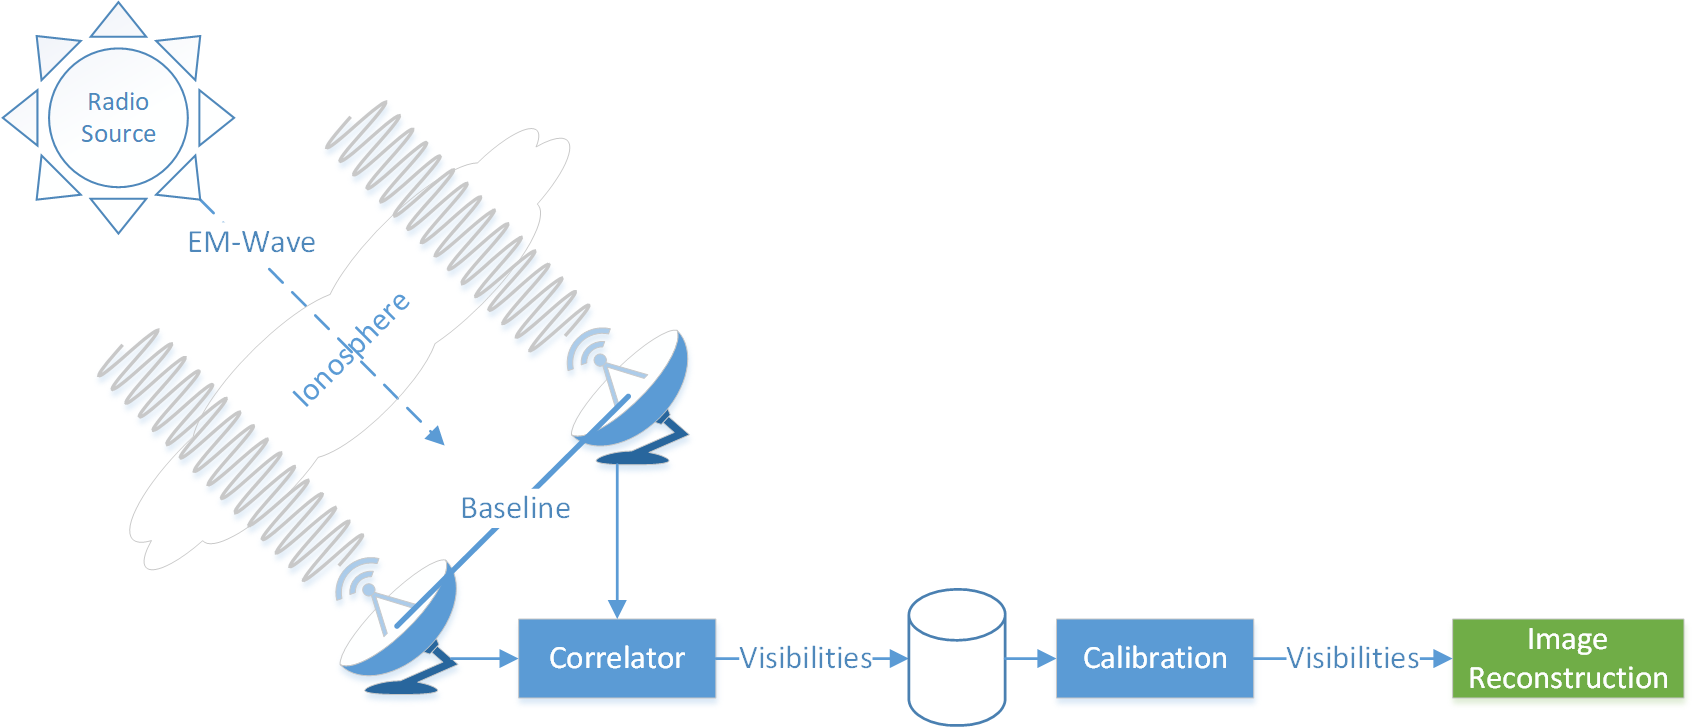
\includegraphics[width=0.80\linewidth]{./chapters/01.intro/system.png}
	\caption{Radio interferometer system}
	\label{intro:system}
\end{figure}

First, the electromagnetic wave gets measured by the different antennas of the interferometer. The measurements of each antenna pair get correlated into a Fourier component (called Visibility in Radio Astronomy). Each antenna pair measures a complex-valued, noisy visibility of the sky. The distance and orientation of the antenna pair relative to the incoming signal, called the baseline, dictates which visibility gets measured. The longer the baseline the higher-order visibility gets measured, resulting in a higher angular resolution. The image \ref{intro:inversefig:uvspace} shows the sampled visibilities in the Fourier space of the MeerKAT interferometer. Every dot is a single measurement. After correlation, the visibility data is saved for later processing.

The calibration step is done after all visibility data has been recorded. This step corrects the amplitude and phase of the measurements for varying antenna sensitivities, pointing errors and other effects. Also, this step removes corrupted data from the measurements. After the calibration step, the visibilities still contain noise.

The last step is responsible for reconstructing an image from the calibrated, noisy visibilities. The figure \ref{intro:inversefig} shows a real-world example of a reconstruction from the MeerKAT radio interferometer. It arrives at the reconstructed image by inverting the measurement equation, and deciding which part of the visibilities is noisy, and which part is the signal. These two problems, handling the noise and inverting the measurement equation, are central to image reconstruction for radio interferometers. They influence both the quality and the runtime costs of the reconstruction.

\begin{figure}[htp]
	% preliminary
	\sbox\twosubbox{%
		\resizebox{\dimexpr.9\textwidth-1em}{!}{%
			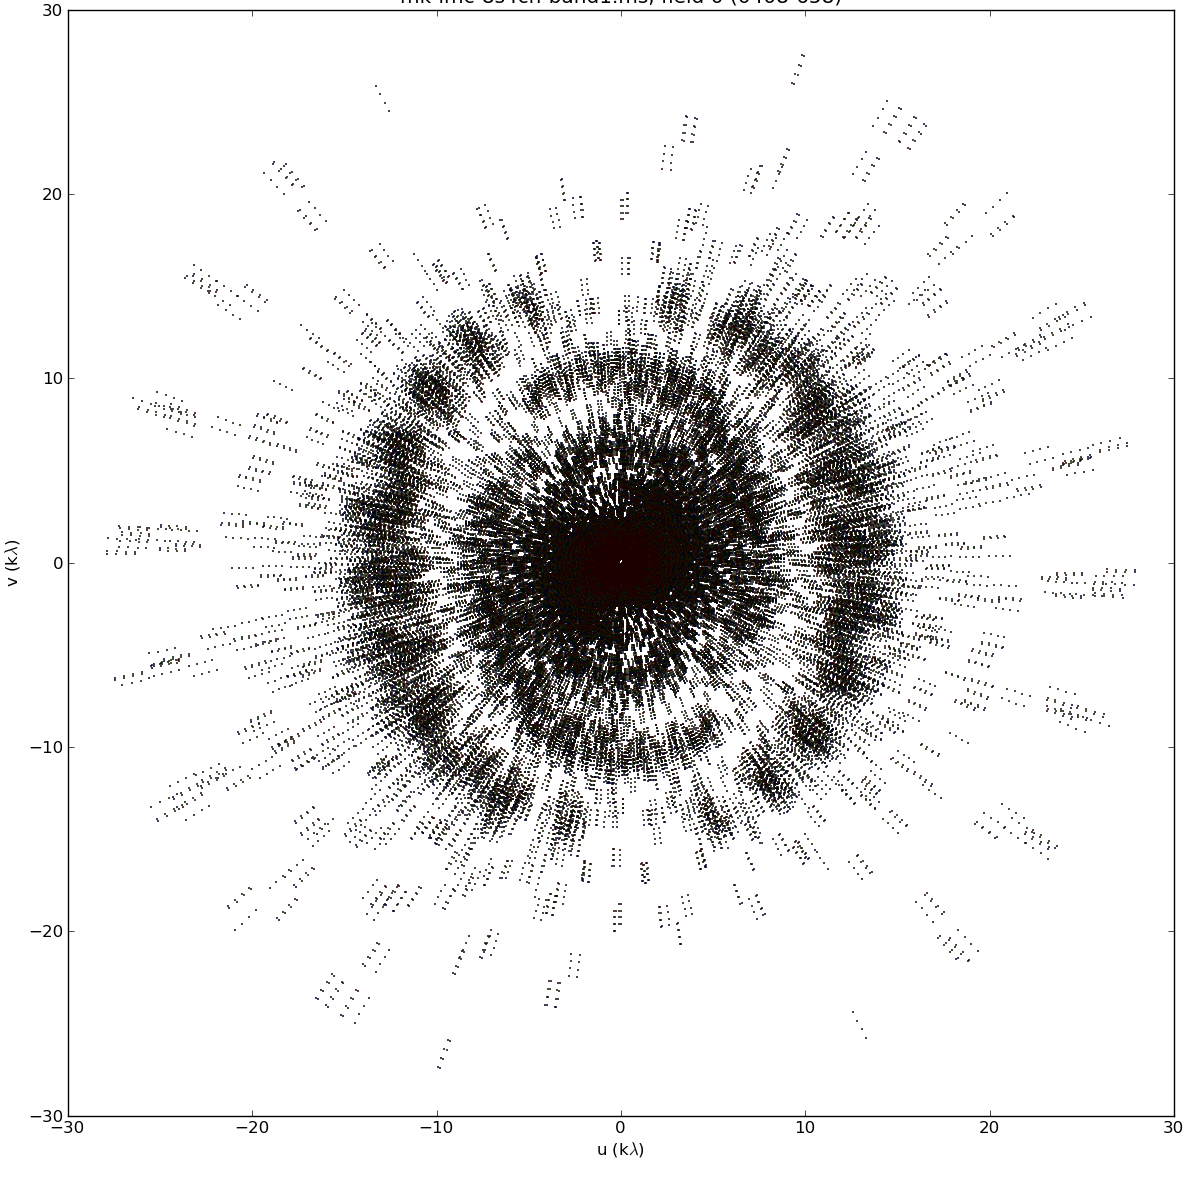
\includegraphics[height=3cm]{./chapters/01.intro/meerkat_uv2.png}%
			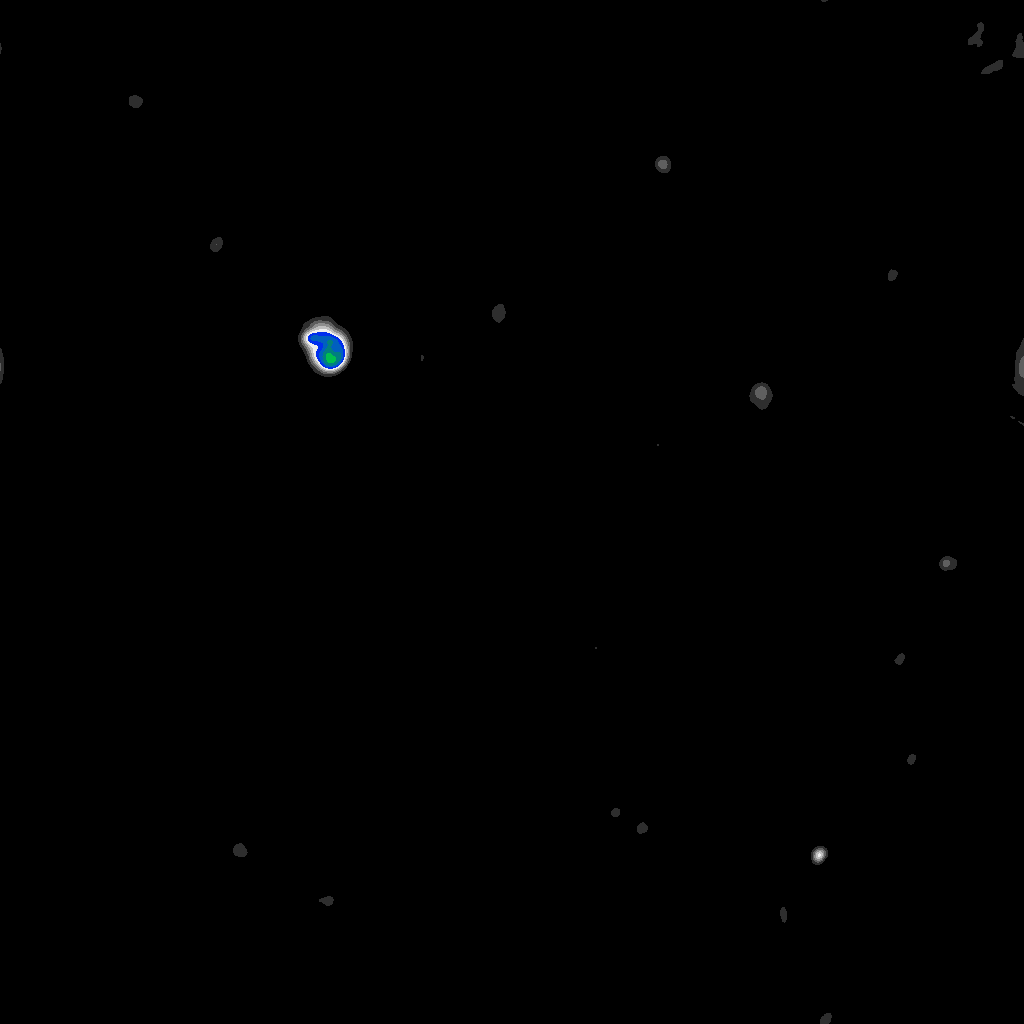
\includegraphics[height=3cm]{./chapters/01.intro/mk2/clean.png}%
		}%
	}
	\setlength{\twosubht}{\ht\twosubbox}
	
	% typeset
	\centering
	\subcaptionbox{Measurements in the Fourier space.\label{intro:inversefig:uvspace}}{%
		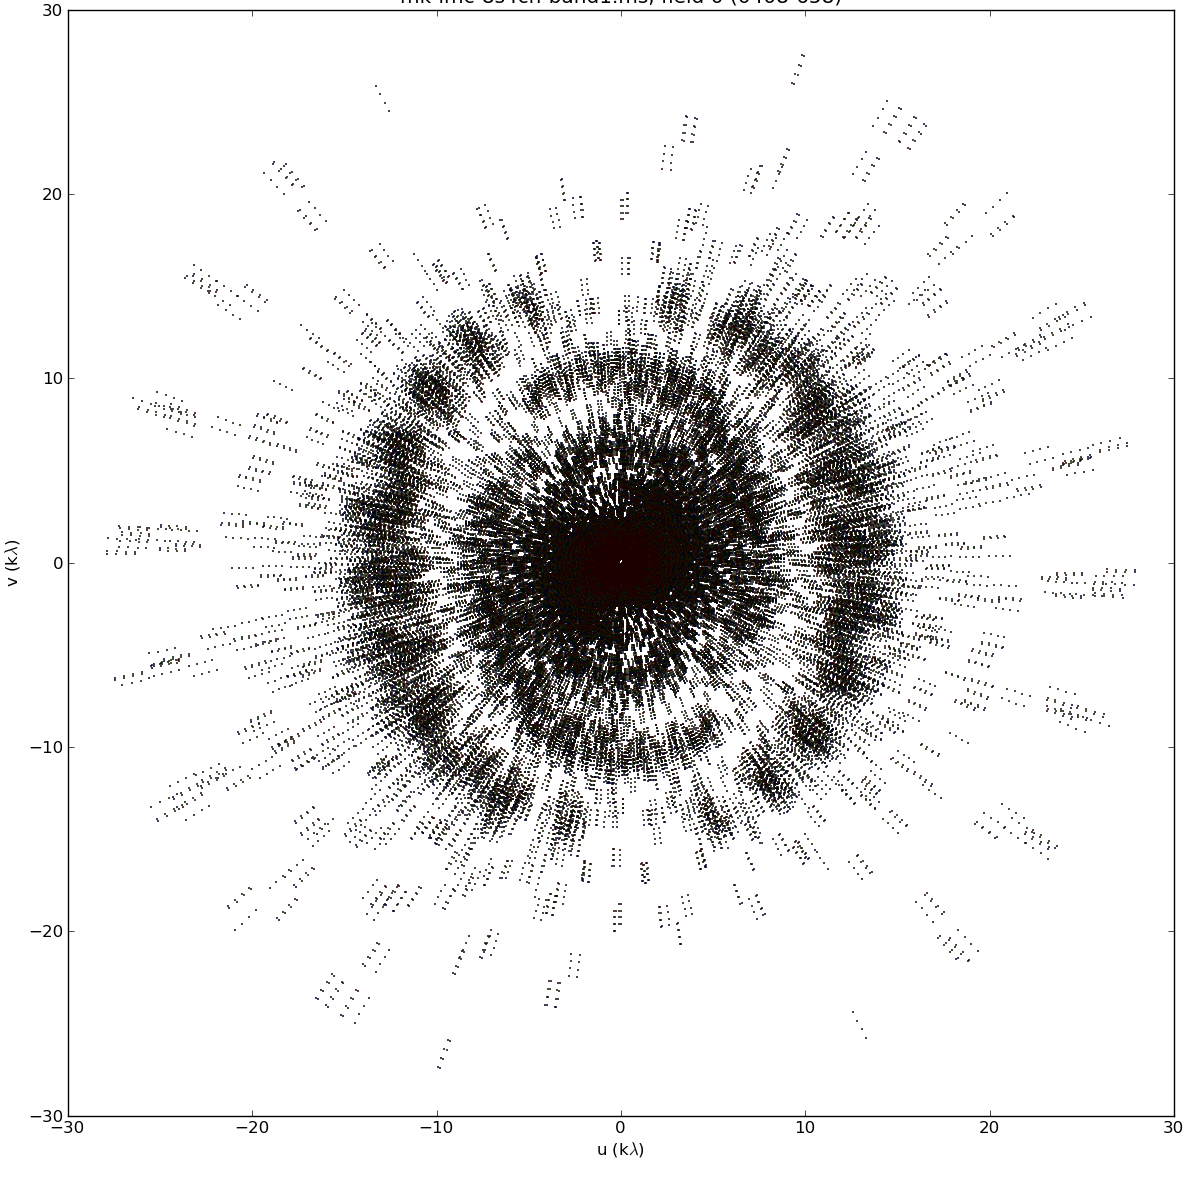
\includegraphics[height=\twosubht]{./chapters/01.intro/meerkat_uv2.png}%
	}\quad
	\subcaptionbox{Reconstructed image.\label{intro:inversefig:reconstruction}}{%
		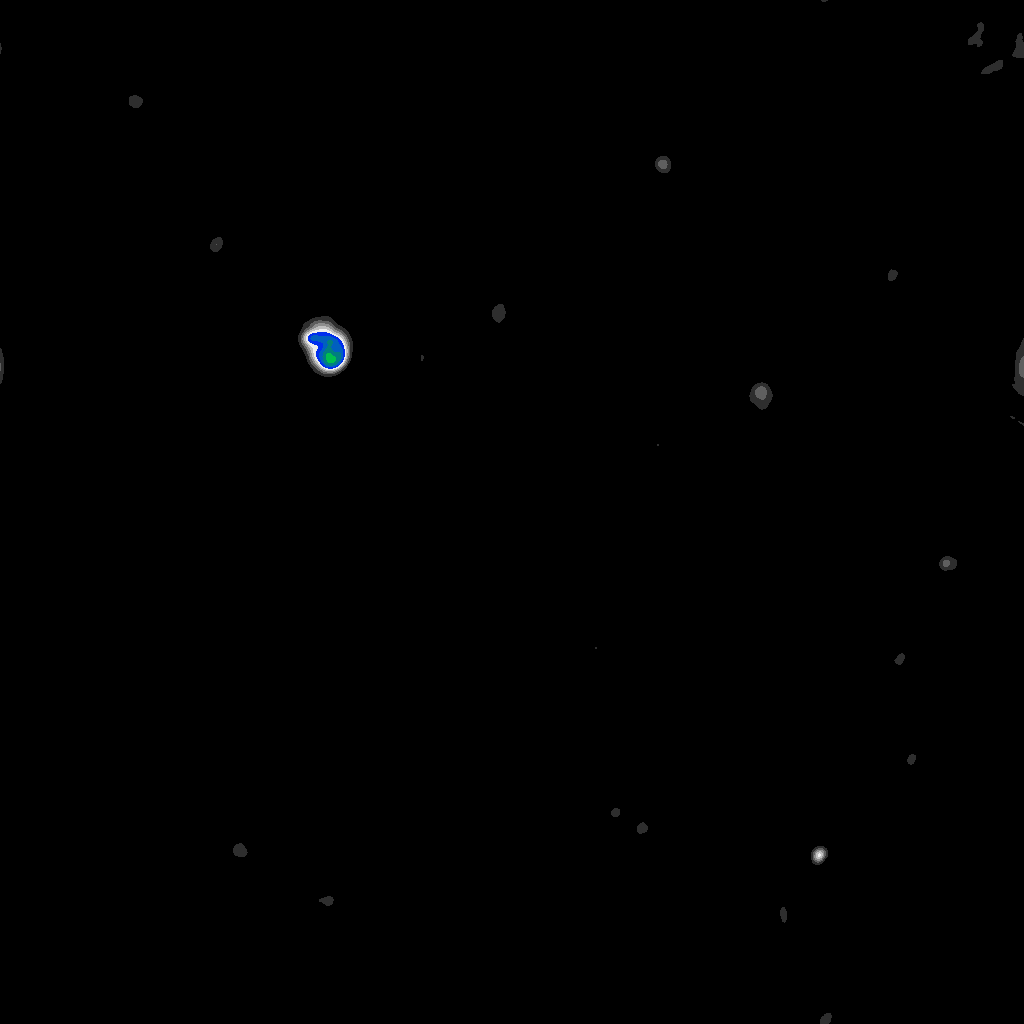
\includegraphics[height=\twosubht]{./chapters/01.intro/mk2/clean.png}%
	}
	\caption{Example of an image reconstruction for visibility measurements of the MeerKAT radio interferometer}\label{intro:inversefig}
\end{figure}


\subsubsection{The measurement equation}
The measurement equation models how the electromagnetic wave gets distorted on its path from the celestial source through the ionosphere and finally through the antenna of the interferometer\cite{smirnov2011revisiting1}. It abstracts all effects we wish to correct in the image reconstruction in one equation. As such, there is no single unified measurement equation for all interferometers, and generally depends on the instrument.

In this project we use the measurement equation \eqref{intro:inverseproblem}. It consists of three parts: The visibility measurements $V(u,v,w)$\footnote{$V$ in the equation \eqref{intro:linear:linear} is a vector. We use the lower-case $v$ to denote the axis in the Fourier space $uvw$, and the upper-case letter to denote the visibility vector.}, the observed image with a normalization factor $\frac{I(x, y)}{c(x, y)}$ and the Fourier Transform $e^{2 \pi i [\ldots]}$. $u$ $v$ and $w$ represent the axes in the Fourier Domain, while the $x$ and $y$ axes represent the angles away from the image center. A pixel in $I(x,y)$ represents how much radio emission was measured from a the direction $x,y$. The image \ref{intro:inversefig:uvspace} shows an example for $V()$, while \ref{intro:inversefig:reconstruction} shows an example for $I()$.

\begin{equation}\label{intro:inverseproblem}
V(u, v, w) = \int\int  \frac{I(x, y)}{c(x, y)}  e^{2 \pi i [ux+vy+ w(c(x, y) - 1)]} \: dx \: dy \:,  \quad c(x,y) = \sqrt{1 - x^2 - y ^2}
\end{equation}

The radio interferometer essentially observes the sky in the Fourier domain. If we want to retrieve the observed sky image $I()$, all we need to do in theory is calculate the inverse Fourier Transform. Note however that the visibilities $V(u,v,w)$ are three dimensional, while the image $I(x,y)$ only has two. Also note that the third component $w$ only depends on the directions $x$ and $y$. In a sense, the Visibilities $V()$ and the image $I()$ have a two dimensional Fourier relationship ($V(u,v,w) = \int\int I(x,y) e^{2 \pi i [ux+vy]} \: dx \: dy$), but with a directionally dependent correction factor $e^{2 \pi i [\ldots +w(c(x, y) - 1)]}$. 

The third component $w$ is an example of a Directionally Dependent Effect (DDE) which have a tendency to increase the runtime costs of the image reconstruction. The $w$-component keeps us from using the Fast Fourier Transform (FFT) for the measurement equation \eqref{intro:inverseproblem}. Research in this area tries to use approximations which lets us use faster algorithms like the FFT, and correct for DDE's accurately enough \cite{veenboer2017image, offringa2014wsclean, pratley2018fast}. In this project, the $w$-correction is the only DDE we handle.


\subsection{System of linear equations}
Even though the Fourier Transform in the measurement equation \eqref{intro:inverseproblem} contains a $w$-correction factor, it is still linear. Even with more complex measurement equations, the relationship between the visibilities $V()$ and the $I()$ remain linear\cite{smirnov2011revisiting}. If we ignore the noise for the sake of demonstration, this means we can represent the measurement equation as a system of linear equations  \eqref{intro:linear:linear}, where $F$ is the Fourier Transform with $w$-correction, $x$ is the image we are searching, $V$ are the calibrated visibilities. To reconstruct the image $x$, we simply need to search for a solution to \eqref{intro:linear:linear}.

\begin{equation}\label{intro:linear:linear}
\underset{x}{find}\quad V - Fx = 0
\end{equation}

Even though we generally have more visibilities than pixels in the reconstruction, which makes \eqref{intro:linear:linear} overdetermined, there is no unique solution to \eqref{intro:linear:linear}. There are potentially many candidate images that solve \eqref{intro:linear:linear}. This makes the image reconstruction for radio interferometers an ill-posed inverse problem. 

The reason why lies in the visibility measurements $V$. When we look back at figure \ref{intro:inversefig:uvspace}, it is clear to see that the interferometer does not sample the visibilities in a uniform way. There are regions with a high sample density. The density decreases when we move further away from the center. In short, the radio interferometer measures an incomplete set of visibilities. The measurements do not contain all the data we require to reconstruct the image. There are potentially many different candidate images that solve equation \eqref{intro:linear:linear}. The observed image is among the candidates, and from the measurements alone we cannot decide which it is. 

Finding the observed image from the incomplete set of visibilities is an ill-posed inverse problem, even if the measurements are noiseless. But as we discussed, radio interferometers produce noisy visibility measurements. We require an image reconstruction algorithm which handles two problems: Finding the observed image from the incomplete measurements and deciding which part of the measurements are noise. 

Both can be handled by including prior information about the image. We know the image contains a mixture of point sources, emissions from stars and other far-away sources concentrated around a single pixel, extended emissions, clouds of hydrogen spanning an area over several arc-seconds. By including prior information, a reconstruction algorithm can find the most-likely image of equation \eqref{intro:linear:linear}. The theory of Compressed Sensing\cite{candes2006robust,donoho2006compressed} gives us a framework for how we can include prior information about the image. 

\subsubsection{The theory of Compressed Sensing}
The theory of Compressed Sensing is a technique for efficient acquisition and reconstruction of signals. For image reconstruction in radio astronomy, it gives us a theoretical framework for analysing reconstruction algorithms. The basic idea of Compressed Sensing reconstruction is: We find a solution to the ill-posed linear system of equations by minimizing an optimization objective \eqref{intro:linear:compressed}, where $x$ is the most likely image we wish to find. A compressed sensing reconstruction algorithm therefore consists of three parts, an objective function, a prior function $P()$ and an optimization algorithm.

\begin{equation}\label{intro:linear:compressed}
\underset{x}{minimize} \: \left \| V - Fx \right \|_2^2 + \lambda P(x)
\end{equation}

The objective consists of two parts, the data term and the regularization term. The data term $\left \| V - Fx \right \|_2^2$ forces the most likely image to be as close to the measurements as possible, and the regularization term $P(x)$ penalizes unlikely images according to our prior function. The parameter $\lambda$ represents how much we penalize unlikely images and by extend, much noise we expect in the reconstruction. The parameter $\lambda$ is either left to the user to define, or an estimation strategy is used \cite{miller1970least}.

The prior function $P()$
Any function we like
From image denoising. L1 L2
Total Variation

Optimization algorithm. Finding the most likely image

Sparse priors. Indicator function. 
L1 norm in a different domain.


The optimum of the objective gives us the most likely image. Bayesian interpretation with prior probability.




Theory of compressed sensing that this works at all. How likely it is that the and that under the right prior P() we are almost guaranteed to find th
Incoherence
RIP, but in practice we have no idea if $F$ fulfills the RIP. But we know it is likely


\subsection{Image reconstruction in practice}\label{intro:major}
We know how to solve the ill-posed image reconstruction problem in theory. We formulate a minimization problem \eqref{intro:linear:compressed}, specify a prior function that capture our prior knowledge, and find the optimum image with an appropriate optimization algorithm. In practice however we have a hard time representing the dense Fourier Transform matrix $F$ in the equation \eqref{intro:linear:compressed}. It is the size of number of visibilities times pixels in the reconstruction. Even older radio interferometers easily produce several million visibilities, with a million pixels in the reconstructed image. We cannot represent $F$ explicitly. However, we can reformulate the image reconstruction \eqref{intro:linear:compressed} as a deconvolution problem, which reduces the dimensions of the measurement $V$ and removes the large Fourier transform matrix $F$ from the minimization objective.

\subsubsection{Reformulating as a deconvolution problem}\label{intro:major:reformulation}
The Fourier transform matrix $F$ in \eqref{intro:linear:compressed} is a product of two operations: The Fourier transform $F$, and the masking operator $M$. The masking operator is a matrix with zero entries for all Fourier components invisible to the instrument. So far, $M$ was implicitly contained in $F$ of \eqref{intro:linear:compressed}. To derive the deconvolution problem, we represent $M$ explicitly. For the sake of demonstration, let us assume our visibility measurements $V(u, v ,w)$ lie on a discrete grid. $V(u, v, w)$ is zero for all components that the interferometer could not measure. We then can represent the transformation from image to visibility space with the Fourier transform $F$ followed by a masking operation $M$, and we arrive at the image reconstruction problem \eqref{intro:major:reformulation:factor}. This is identical to \eqref{intro:linear:compressed}, except for the factorization of $F$.

\begin{alignat}{2}
\text{original:} \quad \underset{x}{minimize}\:& \left \| V - M Fx \right \|_2^2 + &\lambda P(x) \label{intro:major:reformulation:factor}\\ 
\text{in-painting:} \quad\underset{V_2}{minimize}\:& \left \| V - M V_2 \right \|_2^2 + &\lambda P(F^{-1}V_2) \label{intro:major:reformulation:fourier} \\
\text{deconvolution:} \quad \underset{x}{minimize}\:& \left \| I_{dirty} - x * PSF \right \|_2^2 + &\lambda P(x) \label{intro:major:reformulation:deconv}
\end{alignat}

Note that $M$ represents the degradation, the corruption introduced by incomplete sampling in the visibility space. $M$ is the important operator. The measurements $V$, or the reconstructed image $x$ can be in any space we wish. For example, we do not actually need to reconstruct the image in image space. In theory, we can reformulate an equivalent problem \eqref{intro:major:reformulation:fourier}, in which we in-paint the missing visibilities. Or, we can use the Fourier transform on the visibility measurements $V$ and the masking operator $M$, which leads us to the deconvolution problem \eqref{intro:major:reformulation:deconv}. 

Since the deconvolution formulation is vital for the major/minor cycle architecture, we have a closer look at \eqref{intro:major:reformulation:deconv}. The effect of incomplete sampling in Fourier space is equal to a convolution with a Point Spread Function $PSF$ in image space. I.e. $PSF = F^{-1}M$. The measurements are now represented as the "dirty" image, $I_{dirty} = F^{-1}V$. We try to find the deconvolved image $x$, while only knowing the convolution kernel $PSF$ and the convolved, dirty image $I_{dirty}$. This is still an ill-posed inverse problem. We have potentially many different deconvolutions that fit the dirty image, and we search the most likely candidate according to some prior $P(x)$. 

The deconvolution \eqref{intro:major:reformulation:deconv} and the original image reconstruction problem \eqref{intro:linear:compressed} are equivalent. Both arrive at the same result. But the deconvolution problem is easier to handle in practice: $I_{dirty}$ and $PSF$ are generally more compact representations of $V$ and $M$. There is one last issue: Calculating the dirty image from the measurements ($I_{dirty} = F^{-1}V$) again needs the impractically large Fourier transform matrix $F$. This is solved in the major/minor cycle algorithm.

\subsubsection{The major/minor cycle}
The major/minor cycle architecture shown in figure \ref{intro:major:fig} consists of two parts: The minor cycle, which iteratively deconvolves the dirty image with the $PSF$ (it minimizes \eqref{intro:major:reformulation:deconv}). The first half of the major cycle estimates the dirty image. It consists of two steps: the gridding and the Fast Fourier Transformation (FFT). The gridding step takes the incomplete and non-uniformly sampled visibilities and interpolates them on a uniform grid. Then the inverse FFT can be calculated on the interpolated visibilities and we arrive at the dirty image.

\begin{figure}[h]
	\centering
	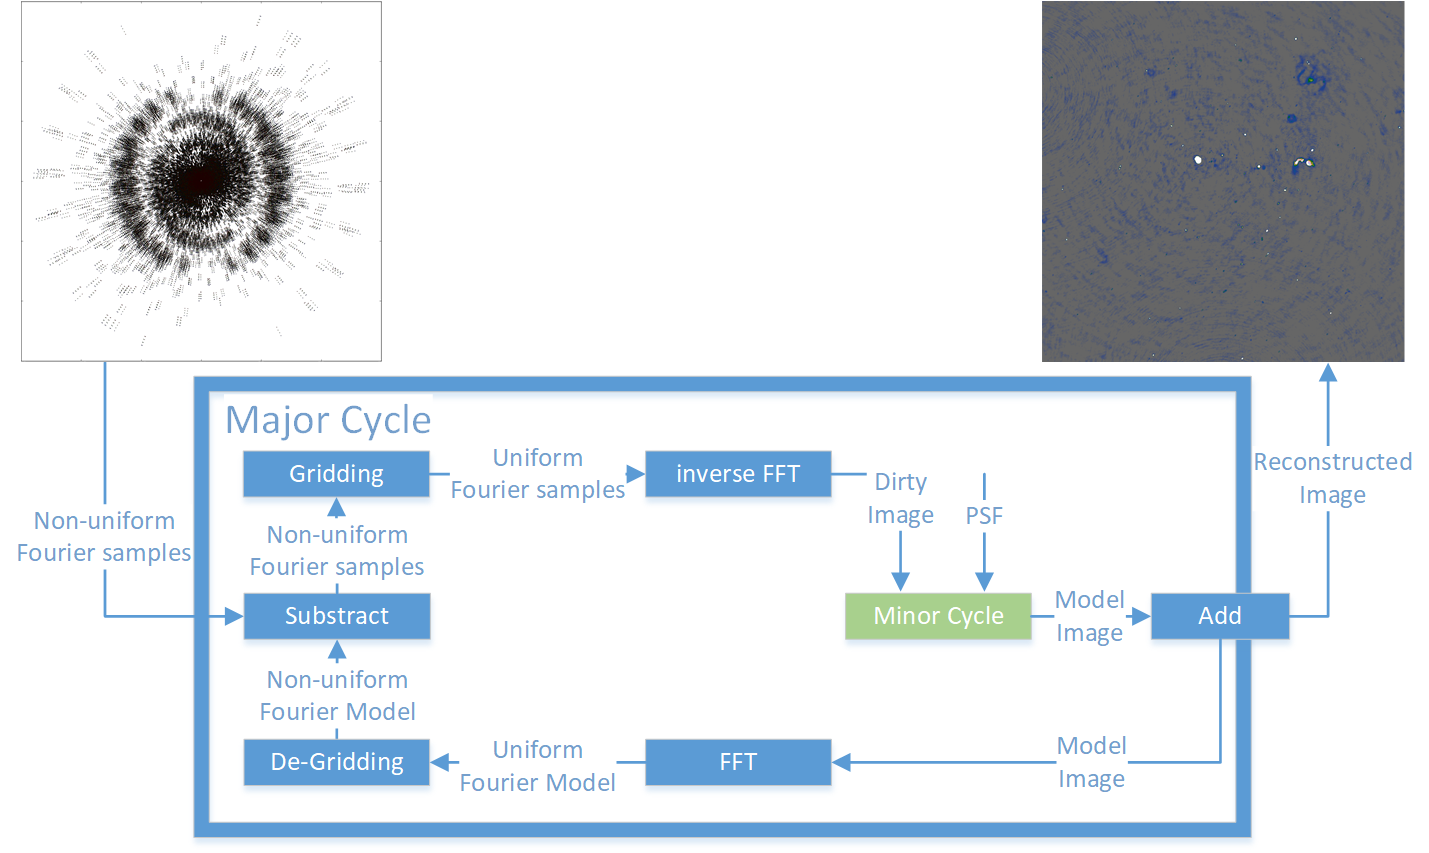
\includegraphics[width=0.90\linewidth]{./chapters/02.hypo/Major-Minor3.png}
	\caption{The Major/Minor Cycle Architecture}
	\label{intro:major:fig}
\end{figure}

Minor Cycle deconvolution. Creates the deconvolved "model" image.

After the Minor Cycle, the second half of the Major Cycle continues. It takes the model image and transforms it back to the original measurement space. FFT and de-gridding. Arriving at the model visibilities.

Then we subtract the model visibilities from the original measurements and start the next Major Cycle with the residual visibilities. The final reconstructed image is the result of several major cycles. Depending on the observation and deconvolution algorithm we require more or fewer major cycles. Expected number around 5

Most expensive operations is the gridding and de-gridding followed by the deconvolution. Gridding is also where we do corrections like the $w$-term. So interpolation becomes specific for the field of radio astronomy.

Depending on the observation, the second most expensive step is the deconvolution.


\subsubsection{Approximations under the major cycle} \label{intro:major:approximations}
Why is the major cycle even necessary. At first glance, it seems like we may be done after the first major cycle. Because the deconvolution problem.

But the $PSF$ is actually just an approximation. The $PSF$ changes over the image.

Plus the gridding also introduces an error which gets reduced over several Major Cycles.

\subsubsection{Alternatives to the major/minor cycle}
Not formulating as a deconvolution, but takes the gridding and FFT step. Fastest approximation. Tends to use many major cycles.
